\begin{solution}
Using the C programming language, we constructed the following finite element method implementation:

\begin{itemize}
\item[] \textbf{main.c} : allows the user to specify his/her values for the function $f$, and boundary conditions for $g$ and $h$.
\item[] \textbf{construct\_matrix.c} : computes $\kappa _{AB}$
\item[] \textbf{gaussian\_quadrature.c} : uses gaussian quadrature to estimate integration values for various functions specified within the file
\item[] \textbf{tridiag\_solver.c} : uses the $lapacke$ library to solve a linear system described by Ax = y for x. 
\end{itemize}

To specify the values for $f$, $g$, and $h$, there is a section in the main function in \textbf{main.c} file, under the section for \texttt{Variable initialization}.

To verify that our solution made sense we graphed our output in a Jupyter notebook that can be found in the same directory as the rest of our code.\\

For $f = 0$, $g = 0$ and $h = 1$, the exact solution will be $u = 1 - x$.

\begin{center}
    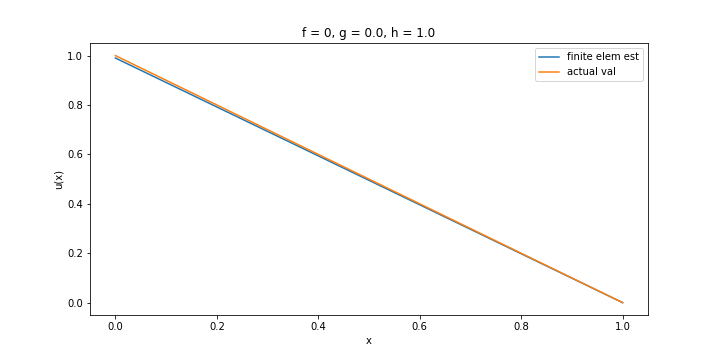
\includegraphics[scale=0.5]{DavidPineiro/f0_g0_h1.png}
\end{center}


\end{solution}
\begin{solution}
For $g = 1$, $h = 1$, $f = 0$, the exact solution will be $u = 2 - x$.

\begin{center}
    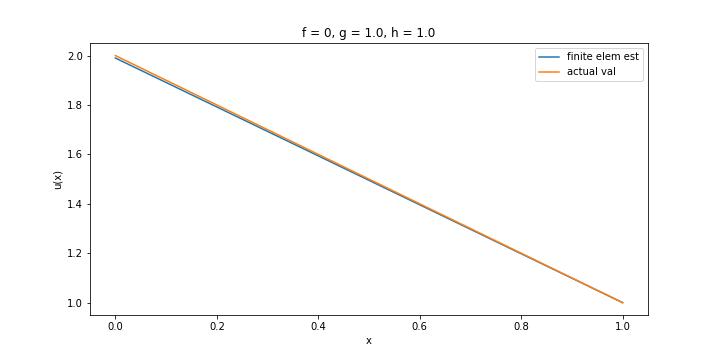
\includegraphics[scale=0.5]{DavidPineiro/f0_g1_h1.png}
\end{center}

For $g = 1$, $h = 1$, and $f = 1$, the exact solution will be $u = 2 - x + \dfrac{1}{2}(\lr{1 - x^{2}})$.

\begin{center}
    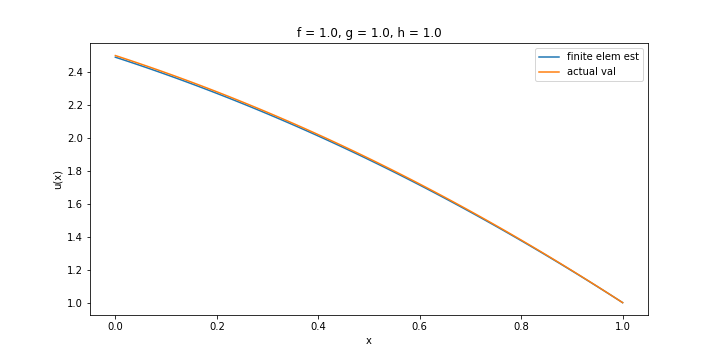
\includegraphics[scale=0.5]{DavidPineiro/f1_g1_h1.png}
\end{center}

Therefore, we verified our solution and have confidence in our code.

\end{solution}